\documentclass[11pt, oneside]{article}   	% use "amsart" instead of "article" for AMSLaTeX format
\usepackage{geometry}                		% See geometry.pdf to learn the layout options. There are lots.
\geometry{letterpaper}                   		% ... or a4paper or a5paper or ... 
%\geometry{landscape}                		% Activate for rotated page geometry
\usepackage[parfill]{parskip}    			% Activate to begin paragraphs with an empty line rather than an indent
\usepackage{graphicx}				% Use pdf, png, jpg, or eps§ with pdflatex; use eps in DVI mode
								% TeX will automatically convert eps --> pdf in pdflatex		
\usepackage{amssymb}
\usepackage{hyperref}
\usepackage{mathtools}
\usepackage{enumerate}
\usepackage{tikz}


\title{Homework 2 \\ CS 5787 Deep Learning \\ Spring 2019}
%\author{John Doe - \texttt{jdoe@cornell.edu}} %Uncomment!!

\date{}					

\begin{document}

\maketitle

\textbf{Due: See Canvas}

\section*{Instructions}

Your homework submission must cite any references used (including articles, books, code, websites, and personal communications).  All solutions must be written in your own words, and you must program the algorithms yourself. \textbf{If you do work with others, you must list the people you worked with.} Submit your solutions as a PDF to Canvas.

Your homework solution must be typed, and we suggest you do this using \LaTeX. Homework must be output to PDF format. I suggest using \url{http://overleaf.com}  to create your document. Overleaf is free and can be accessed online.

Your programs must be written in  Python. The relevant code to the problem should be in the PDF you turn in. If a problem involves programming, then the code should be shown as part of the solution to that problem. One easy way to do this in \LaTeX \, is to use the verbatim environment, i.e., \textbackslash begin\{verbatim\} YOUR CODE \textbackslash end\{verbatim\}

If you have forgotten your linear algebra, you may find  \textit{The Matrix Cookbook} useful, which can be readily found online. You may wish to use the program \textit{MathType}, which can easily export equations to AMS \LaTeX \, so that you don't have to write the equations in \LaTeX \, directly: \url{http://www.dessci.com/en/products/mathtype/}

\sloppy
\textbf{If told to implement an algorithm, don't use a toolbox, or you will receive no credit. Do not post your code to a public web repository (e.g., GitHub).}

%%%%%%%%%%%%%%%%%%%%%%%%%%%%%%%%%%%%%%%%%%%%%

\section*{Problem 1 - Using a Pre-Trained CNN}
For this problem you must use PyTorch.


\subsection*{Part 1 - Using Pre-Trained Deep CNN (5 points)}
For this problem you will use a CNN that has been trained on ImageNet-1k. Choose the pre-trained model of your choice (e.g., VGG-16, VGG-19, ResNet-18, ResNet-152, etc.). Run it on \texttt{peppers.jpg}. Output the top-3 predicted categories and the probabilities.

Make sure to list the deep CNN model you used. Make sure to pre-process the input image appropriately. Look at the toolbox documentation for the pre-trained model you use to determine how to do this. 

\textbf{Solution:} \\



\subsection*{Part 2 - Visualizing Feature Maps (5 points)}

Write code to visualize the feature maps in the network as images. You will likely need to normalize the values between 0 and 1 to do this. %See this: https://stackoverflow.com/questions/13384653/imshow-extent-and-aspect/13390798#13390798

Choose five interesting feature maps from early in the network, five from the the middle of the network, and and five close to the end of the network. Display them to us and discuss  the structure of the feature maps. Try to find some that are interpretable, and discuss the challenges in doing so. 

\textbf{Solution:} \\


%----------------------
\section*{Problem 2 - Transfer Learning with a Pre-Trained CNN (20 points)}

For this problem you must use PyTorch. We will do image classification using the Oxford Pet Dataset. The dataset consists of 37 categories with about 200 images in each of them. You can find the dataset here: \url{http://www.robots.ox.ac.uk/~vgg/data/pets/}


Rather than using the final `softmax' layer of the CNN as output to make predictions as we did in problem 1, instead we will use the CNN as a feature extractor to classify the Pets dataset. For each image, grab features from the last hidden layer of the neural network, which will be the layer \textbf{before} the 1000-dimensional output layer (around 2000--6000 dimensions). You will need to resize the images to a size compatible with your network (usually $224 \times 224 \times 3$). If your CNN model is using ReLUs, then you should grab the output just after the ReLU (so all values will be non-negative). 

After you extract these features for all of the images in the dataset, normalize them to unit length by dividing by the $L_2$ norm. Train a linear classifier of your choice\footnote{You could use the softmax classifier you implemented for homework 1 or any toolbox you prefer.} with the training CNN features, and then classify the test CNN features. Report mean-per-class accuracy and discuss the classifier you used. 



\textbf{Solution:}\\



%--------------------------------------------
\section*{Problem 3 - Training a Small CNN}

\section*{Part 1 (30 points)}

For this problem you must use a toolbox. Train a CNN with three hidden convolutional layers that use the ReLU activation function. Use 64 $11\times 11$ filters for the first layer, followed by $2 \times 2$ max pooling (stride of 2). The next two convolutional layers will use 128 $3 \times 3$ filters followed by the ReLU activation function. Prior to the softmax layer, you should have an average pooling layer that pools across the preceding feature map. Do not use a pre-trained CNN.

Train your model using all of the CIFAR-10 training data, and evaluate your trained system on the CIFAR-10 test data.

Visualize all of the $11 \times 11 \times 3$ filters learned by the first convolutional layer as an RGB image array (I suggest making a large RGB image that is made up of each of the smaller images, so it will have 4 rows and 16 columns). This visualization of the filters should be similar to the ones we saw in class. Note that you will need to normalize each filter by contrast stretching to do this visualization, i.e., for each filter subtract the smallest value and then divide by the new largest value.

Display the training loss as a function of epochs. What is the accuracy on the test data? How did you initialize the weights? Discuss your architecture and hyper-parameters.

\textbf{Solution:}\\

IMAGE SHOWING THE FILTERS \\
TRAINING LOSS AS FUNCTION OF EPOCHS \\
TEST DATA ACCURACY \\
WEIGHT INITIALIZATION INFORMATION \\
DESCRIBE HYPER-PARAMETERS \\

\section*{Part 2 (20 points)}

Using the same architecture as in part 1, add in batch normalization between each of the hidden layers. Compare the training loss with and without batch normalization as a function of epochs. What is the final test error? Visualize the filters. 

\textbf{Solution:}\\



\section*{Part 3 (10 points)}
Can you do better with a deeper and better network architecture? Optimize your CNN's architecture to improve performance. You may get significantly better results by using smaller filters for the first convolutional layer. Describe your model's architecture and your design choices. What is your final accuracy?

Note: Your model should perform better than the one in Part 1 and Part 2.

\textbf{Solution:}\\





%%%%%%%%%%%%%%%%%%%%%%%%%%%%%%%%%%%%%%%%%%%%%
\section*{Problem 4 - Fooling Convolutional Neural Networks}

In this problem you will fool the pre-trained convolutional neural network of your choice. One of the simplest ways to do this is to add a small amount of adversarial noise to the input image, which causes the correct predicted label $y_{true}$ to switch to an incorrect adversarial label $y_{fool}$, despite the image looking the same to our human visual system. 


\subsection*{Part 1 (20 points)}

More formally, given an input image $\mathbf{X}$, an ImageNet pre-trained network will give us $P\left( {y|{\mathbf{X}}} \right)$, which is a probability distribution over labels and the predicted label can be computed using the argmax function. We assume the network has been trained to correctly classify $\mathbf{X}$. To create an adversarial input, we want to find ${{\mathbf{\hat X}}}$ such that  ${{\mathbf{\hat X}}}$ will be misclassified as $y_{fool}$. To ensure that  ${{\mathbf{\hat X}}}$ does not look radically different from  $\mathbf{X}$ we impose a constraint on the distance between the original and modified images, i.e., $\left\| {{\mathbf{X}} - {\mathbf{\hat X}}} \right\|_\infty   \leqslant \epsilon ,$ where $\epsilon$ is a small positive number. This model can be trained using backpropagation to find the adversarial example, i.e.,
\[
{\mathbf{\hat X}} = \arg \min _{{\mathbf{X'}}} \left( {Loss\left( {{\mathbf{X'}},y_{fool} } \right) + \frac{\lambda }
{2}\left\| {{\mathbf{X'}} - {\mathbf{X}}} \right\|_\infty  } \right),
\]
where $\lambda > 0$ is a hyperparameter and $\left\| \cdot \right\|_\infty$ denotes the infinity norm for tensors.

To do this optimization, you can begin by initializing ${\mathbf{X'}} \leftarrow {\mathbf{X}}$. Then, repeat the following two steps until you are satisfied with the results (or convergence):
\[
\begin{gathered}
  {\mathbf{X'}} \leftarrow {\mathbf{X'}} + \lambda \frac{\partial }
{{\partial {\mathbf{X'}}}}P\left( {y_{fool} |{\mathbf{X'}}} \right) \hfill \\
  {\mathbf{X'}} \leftarrow {\text{clip}}\left( {{\mathbf{X'}},{\mathbf{X}} - \epsilon ,{\mathbf{X}} + \epsilon } \right) \hfill \\ 
\end{gathered} 
\]
where the \texttt{clip} function `clips' the values so that each pixel is within $ \epsilon$ of the original image. You may use the neural network toolbox of your choice to do this optimization, but we will only provide help for PyTorch. You can read more about this approach here: \url{https://arxiv.org/pdf/1707.07397.pdf}. Note that the details are slightly different.



Demonstrate your method on four images. The first image should be `peppers,' which was used in an earlier assignment. Show that you can make the network classify it as a space shuttle (ImageNet class id 812). You can choose the other three photos, but ensure that they contain an ImageNet object and make the network classify it as a different class. Ensure that the pre-trained CNN that you use outputs the correct class as the most likely assignment and give its probability. Then, show the `noise image' that will be added to the original image. Then, show the noise+original image along with the new most likely class and the new largest probability. The noise+original image should be perceptually indistinguishable from the original image (to your human visual system). You may use the ImageNet pre-trained CNN of your choice (e.g., VGG-16, ResNet-50, etc.), but mention the pre-trained model that you used. You can show your results as a $4 \times 3$ array of figures, with each row containing original image (titled with  most likely class and probability), the adversarial noise, and then the new image (titled with  most likely class and probability).




\textbf{Solution:}\\

%%%%%%%%%%%%%%%%%%%%%%%%%%%%%
\subsection*{Part 2 (10 points)}
The method we deployed to make adversarial examples is not robust to all kinds of transformations. To examine the robustness of this, take the four adversarial images you created in part 1 and show how the following image manipulations affect the predicted class probabilities: mirror reflections (flip the image), a crop that contains about 80\% of the original object, a 30 degree rotation, and converting the image to grayscale and then replicating the three gray channels. Show the modified adversarial images and title them with the new most likely class and probabilities. Discuss the results and why you think it did or did not work in each case. 


\textbf{Solution:}\\




%%%%%%%%%%%%%%%%%%%%%%%%%%%%%%%%%%%%
\section*{Problem 5 - Recurrent Neural Networks (10 points)}
Recurrent neural networks (RNNs) are universal Turing machines as long as they have enough hidden units. In the next homework assignment we will cover using RNNs for large-scale problems, but in this one you will find the parameters for an RNN that implements binary addition. Rather than using a toolbox, you will find them by hand.

The input to your RNN will be two binary numbers, starting with the \emph{least} significant bit. You will need to pad the largest number with an additional zero on the left side and you should make the other number the same length by padding it with zeros on the left side. For instance, the problem
\[
100111 + 110010 = 1011001
\]
would be input to your RNN as:
\begin{itemize}
\item Input 1: 1, 1, 1, 0, 0, 1, 0
\item Input 2: 0, 1, 0, 0, 1, 1, 0
\item Correct output: 1, 0, 0, 1, 1, 0, 1
\end{itemize}

The RNN has two input units and one output unit. In this example, the sequence of inputs and outputs would be:

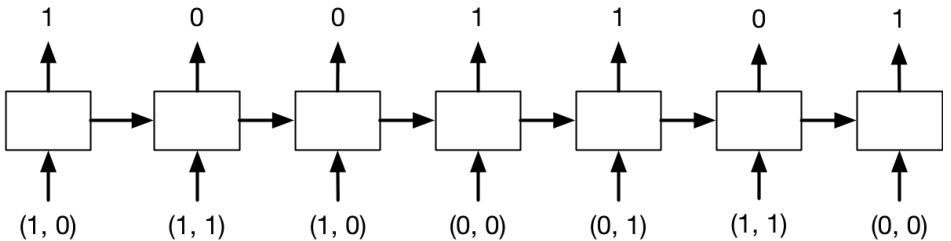
\includegraphics[width=\linewidth]{example.png}

The RNN that implements binary addition has three hidden units, and all of the units use the following non-differentiable hard-threshold activation function
\[
\sigma \left( a \right) = \left\{ {\begin{array}{*{20}c}
   1 & {{\text{if }}a > 0}  \\
   0 & {{\text{otherwise}}}  \\

 \end{array} } \right.
\]

\begin{figure}
\centering
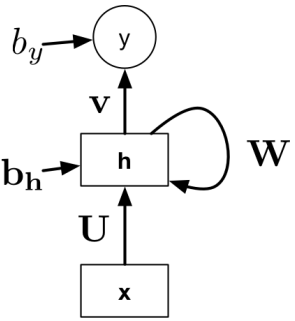
\includegraphics[width = .3\linewidth]{rnn.png}
\end{figure}

The equations for the network are given by
\[
\begin{gathered}
  y_t  = \sigma \left( {{\mathbf{v}}^T {\mathbf{h}}_t  + b_y } \right) \hfill \\
  {\mathbf{h}}_t  = \sigma \left( {{\mathbf{Ux}}_t  + {\mathbf{Wh}}_{t - 1}  + {\mathbf{b}}_{\mathbf{h}} } \right) \hfill \\ 
\end{gathered} 
\]
where $\mathbf{x}_t \in \mathbb{R}^2$, $\mathbf{U} \in \mathbb{R}^{3 \times 2} $, $\mathbf{W} \in \mathbb{R}^{3 \times 3} $,  $\mathbf{b}_\mathbf{h} \in \mathbb{R}^{3}$,  $\mathbf{v} \in \mathbb{R}^3$, and $b_y \in \mathbb{R}$


\subsection*{Part 1 - Finding Weights }

Before backpropagation was invented, neural network researchers using hidden layers would set the weights by hand. Your job is to find the settings for all of the parameters by hand, including the value of $\mathbf{h}_0$. Give the settings for all of the matrices, vectors, and scalars to correctly implement binary addition.

Hint: Have one hidden unit activate if the sum is at least 1, one hidden unit activate if the sum is at least 2, and one hidden unit if it is 3.


\textbf{Solution:} \\



%---------------
\section*{Code Appendix}


\end{document}  